% Fig. 1: the experimental design. The image tiles are real data rendered by
% make_fig_framework.py (one CREMA-D clip in all four conditions, and a slice of
% the feature table); everything else is drawn here.
\begin{figure*}[!t]
\centering
\definecolor{stA}{HTML}{2B5C8A}
\definecolor{stB}{HTML}{6A3D9A}
\definecolor{stC}{HTML}{1B7F79}
\definecolor{stD}{HTML}{C0571B}
\definecolor{nullc}{HTML}{B8860B}
\begin{tikzpicture}[x=1mm, y=1mm, font=\scriptsize,
  panel/.style={rounded corners=2.5pt, line width=0.6pt},
  badge/.style={circle, fill=#1, text=white, font=\bfseries\scriptsize,
                inner sep=0pt, minimum size=4.2mm},
  head/.style={font=\bfseries\scriptsize, anchor=west, text=#1},
  tile/.style={inner sep=0pt, outer sep=0pt},
  tcap/.style={font=\tiny, inner sep=0.5pt, align=center},
  flow/.style={-{Latex[length=2.6mm,width=2.4mm]}, line width=1.6pt, black!45},
]
% ------------------------------------------------------------ stage panels
\fill[stA!7, panel] (0,0) rectangle (34,-49);
\fill[stB!7, panel] (38,0) rectangle (100,-49);
\fill[stC!7, panel] (104,0) rectangle (140,-49);
\fill[stD!7, panel] (144,0) rectangle (181,-49);
\foreach \x/\c/\n/\t in {0/stA/1/Stimuli, 38/stB/2/Four renderings,
                          104/stC/3/Named features, 144/stD/4/Two protocols}{
  \node[badge=\c] at (\x+3.6,-3.6) {\n};
  \node[head=\c] at (\x+6.4,-3.6) {\t};
}
\draw[flow] (34.3,-24) -- (37.7,-24);
\draw[flow] (100.3,-24) -- (103.7,-24);
\draw[flow] (140.3,-24) -- (143.7,-24);

% ------------------------------------------------------------ 1 stimuli
\node[tile] (wave) at (17,-12) {
\includegraphics[width=28mm]{figs/fw_wave.png}};
\node[tcap, below=0.6mm of wave] (corp)
  {\textbf{CREMA-D}\\7{,}441 clips $\cdot$ 91 actors\\12 sentences $\cdot$ 6 emotions};
\draw[-{Latex[length=1.6mm]}, stA, line width=0.7pt] (17,-27) -- (17,-31);
\node[draw=stA, fill=white, rounded corners=1.5pt, tcap, minimum width=28mm,
      inner sep=1.4pt] at (17,-37.5)
  {\textbf{canonical reference} $x$\\\SI{16}{\kilo\hertz} mono PCM\\EBU R128,
   $-23$\,LUFS};

% ------------------------------------------------------------ 2 renderings
% 2x2 grid of spectrograms of the same clip, one shared dB scale
\def\tw{27}
\foreach \cx/\cy/\f/\nm/\ds in {
    53.5/-12.5/ref/ref/uncompressed WAV,
    84.5/-12.5/mp3_64/mp3\_64/{MP3 64\,kb/s},
    53.5/-32.5/mp4_aac64/mp4\_aac64/{AAC 64\,kb/s in MP4},
    84.5/-32.5/roundtrip_wav/roundtrip\_wav/{same AAC, WAV container}}{
  \node[tile, draw=black!35, line width=0.3pt] (s-\f) at (\cx,\cy)
    {\includegraphics[width=\tw mm, height=13mm]{figs/fw_spec_\f.png}};
  \node[tcap, anchor=north] at (s-\f.south) {\textbf{\ttx{\nm}}\\\ds};
}
% MP3: the top band is gone
\draw[red!80!black, densely dashed, line width=0.7pt]
  ($(s-mp3_64.north west)+(0.3,-0.3)$) rectangle ($(s-mp3_64.north east)+(-0.3,-3.6)$);
\node[tcap, fill=white, text=red!75!black, font=\tiny\bfseries, anchor=north east,
      rounded corners=1pt] at ($(s-mp3_64.north east)+(-0.6,-4.0)$)
  {6--8\,kHz lost};
% AAC: priming delay
\node[tcap, fill=white, text=stB, font=\tiny\bfseries, anchor=north west,
      rounded corners=1pt] at ($(s-mp4_aac64.north west)+(0.6,-0.6)$)
  {+32.7\,ms priming};
% roundtrip: same codec output, different container
\node[circle, fill=white, draw=stB, line width=0.6pt, inner sep=0.4pt,
      font=\scriptsize\bfseries, text=stB] at (69,-32.5) {$\equiv$};

% ------------------------------------------------------------ 3 features
\node[tile, draw=black!35, line width=0.3pt] (feat) at (122,-17)
  {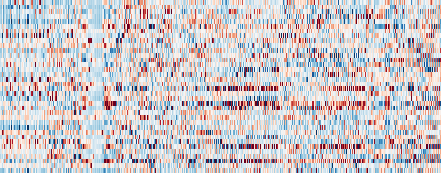
\includegraphics[width=32mm, height=15mm]{figs/fw_features.png}};
\node[tcap, anchor=south, text=black!60] at (feat.north) {36 clips $\times$ 434 descriptors};
% family strip, widths proportional to column counts (114/240/56/24)
\begin{scope}[shift={(feat.south west)}]
  \fill[stA!70]  (0,-0.6) rectangle (8.43,-2.2);
  \fill[stB!70]  (8.43,-0.6) rectangle (26.13,-2.2);
  \fill[stC!80]  (26.13,-0.6) rectangle (30.27,-2.2);
  \fill[stD!80]  (30.27,-0.6) rectangle (32,-2.2);
  \node[tcap, anchor=north] at (4.2,-2.3) {spectral\\114};
  \node[tcap, anchor=north] at (17.3,-2.3) {cepstral\\240};
  \node[tcap, anchor=north] at (29.3,-2.3) {prosodic 56\\chroma 24};
\end{scope}
\node[tcap, anchor=north] at (122,-36.5)
  {\emph{e.g.}\ \ttx{prosody\_intensity\_std},\\\ttx{spectral\_contrast\_6\_mean}};
\node[tcap, anchor=north, text=stC] at (122,-42.5)
  {\textbf{speaker-independent split}\\60/11/20 actors};

% ------------------------------------------------------------ 4 protocols
\node[draw=stD, fill=white, rounded corners=1.5pt, tcap, minimum width=33mm,
      inner sep=1.4pt] (mis) at (162.5,-12.5)
  {\textbf{mismatch}\ \ fit on \ttx{ref}, serve all\\
   \emph{what a deployed model suffers}};
\node[draw=stD, fill=white, rounded corners=1.5pt, tcap, minimum width=33mm,
      inner sep=1.4pt] (mat) at (162.5,-22.5)
  {\textbf{matched}\ \ fit and serve in $c$\\
   \emph{what survives the codec}};
% evidence read off the fitted models: an exact tree and an attribution ranking
\begin{scope}[shift={(151,-31)}, every node/.style={circle, fill=stD,
              inner sep=0pt, minimum size=1.3mm}]
  \node (r) at (0,0) {};
  \node (a) at (-3,-3.5) {}; \node (b) at (3,-3.5) {};
  \node (a1) at (-4.5,-7) {}; \node (a2) at (-1.5,-7) {};
  \node (b1) at (1.5,-7) {};  \node (b2) at (4.5,-7) {};
  \draw[stD, line width=0.5pt] (r)--(a) (r)--(b) (a)--(a1) (a)--(a2)
                               (b)--(b1) (b)--(b2);
\end{scope}
\node[tcap] at (151,-41.5) {entropy tree\\(exact)};
\begin{scope}[shift={(168,-30.5)}]
  \foreach \w [count=\i] in {11,8.5,6.5,5,3.5,2.5}{
    \fill[stD!75] (0,-\i*1.25) rectangle (\w,-\i*1.25+0.85);
  }
\end{scope}
\node[tcap] at (174,-41.5) {attribution\\ranking};

% ------------------------------------------------------------ null band
% A gauge of top-25 retention (paired draws, Table~\ref{tab:paired}):
% x = 58 + (25 - r) * 7.5, so displacement grows to the right.
\fill[nullc!10, panel] (0,-52) rectangle (181,-68);
\node[badge=nullc] at (3.6,-55.6) {5};
\node[head=nullc!80!black] at (6.4,-55.6) {Null calibration};
\node[anchor=north west, tcap, align=left] at (2,-59)
  {A codec effect is the \emph{excess} over an\\
   informationally empty floor, not the raw\\
   drop from a clean refit.};
\node[tcap, anchor=east, text=black!60] at (57,-61) {top-25 kept};
\draw[black!45, line width=0.5pt] (58,-61) -- (171,-61);
\fill[nullc!45, rounded corners=1pt] (64.4,-60.1) rectangle (127,-61.9);
\fill[stD!45,  rounded corners=1pt] (127,-60.1) rectangle (165.6,-61.9);
\node[tcap, anchor=south, text=nullc!70!black] at (95.7,-59.6)
  {\textbf{generic sensitivity}: 8.4 descriptors};
\node[tcap, anchor=south, text=stD!85!black] at (146.3,-59.6)
  {\textbf{codec excess}: MP3 3.3, AAC 5.2};
\foreach \x/\c/\lab in {64.4/black!55/{refit floor\\24.2},
                        127/nullc!85!black/{\textbf{empty re-wrap}\\15.8},
                        151.4/stD/{MP3\\12.6},
                        165.6/stD/{AAC\\10.7}}{
  \fill[\c, draw=white, line width=0.5pt] (\x,-61) circle (1.05);
  \node[tcap, anchor=north] at (\x,-62.3) {\lab};
}
\draw[-{Latex[length=1.8mm]}, nullc!85!black, line width=0.8pt]
  (162.5,-49.3) -- (162.5,-52.2);
\end{tikzpicture}
\caption{Experimental design. The spectrograms show one CREMA-D clip in each of the four conditions.}
\label{fig:framework}
\end{figure*}
